\documentclass[10pt,fleqn]{article} % Default font size and left-justified equations
\usepackage[%
    pdftitle={Modélisation dynamique},
    pdfauthor={Xavier Pessoles}]{hyperref}

\input{style/new_style}
\input{style/macros_SII}
\usepackage{bm}
\fichetrue
\fichefalse

\proftrue
%\proffalse

%\tdtrue
\tdfalse

\courstrue
%\coursfalse



% -------------------------------------
% Déclaration des titres
% -------------------------------------

\def\discipline{Sciences \\Industrielles de \\ l'Ingénieur}
\def\xxtete{Sciences Industrielles de l'Ingénieur}

\def\classe{\textsf{PSI$\star$ -- MP}}
\def\xxnumpartie{Cycle 04}
\def\xxpartie{Modéliser le comportement des systèmes mécaniques dans le but d'établir une loi de comportement ou de déterminer des actions mécaniques en utilisant le PFD}

\def\xxnumchapitre{Chapitre 1 \vspace{.2cm}}
\def\xxchapitre{\hspace{.12cm} Introduction à la dynamique du solide indéformable}

\def\xxposongletx{2}
\def\xxposonglettext{1.45}
\def\xxposonglety{19}%16

\def\xxonglet{\textsf{Cycle 04}}

\def\xxactivite{Cours}
\def\xxauteur{\textsl{Xavier Pessoles}}

\def\xxcompetences{%
\textsl{%
\textbf{Savoirs et compétences :}\\
\begin{itemize}[label=\ding{112},font=\color{ocre}] 
\item \textit{Res1.C2} : principe fondamental de la dynamique;
\item \textit{Res1.C1.SF1} : proposer une démarche permettant la détermination de la loi de mouvement.
\end{itemize}
}}
		
\def\xxfigures{
\includegraphics[width=4cm]{images/newton}%images/prot_01
%\\

 \textit{Isaac Newton -- 1643 - 1727.}
}%figues de la page de garde

\def\xxpied{%
Cycle 04 -- Modéliser le comportement des systèmes mécaniques\\% afin de valider leurs performances.\\
Chapitre 1 -- \xxactivite%
}

\setcounter{secnumdepth}{5}
%---------------------------------------------------------------------------


\begin{document}
\chapterimage{png/Fond_CIN}
\input{style/new_pagegarde}
\setlength{\columnseprule}{.1pt}

\vspace{2cm}
\pagestyle{fancy}
\thispagestyle{plain}


\section{Introduction}
\begin{obj} ~\\
L'objectif de ce cycle est triple. L'étude dynamique des systèmes de solide permet de 
\begin{itemize}
\item déterminer les actions mécaniques dans les liaisons en tenant compte des masses (et des répartitions de masses) des pièces ou des classes d'équivalence cinématique;
\item dimensionner les actionneurs permettant d'actionner un système; 
\item déterminer les équations de mouvement.
\end{itemize}
\end{obj}
%\subsection{Définitions}


\begin{definition}[Référentiel galiléen]
Un \textbf{référentiel galiléen} se définit à partir d'une repère spatial (orthonormé direct $\quadruplet{O_g}{\overrightarrow{x_g}}{\overrightarrow{y_g}}{\overrightarrow{z_g}}$ et d'une base de temps ($t$) et est animé d'un mouvement de \textbf{translation rectiligne uniforme} (à vitesse constante) par rapport à un référentiel absolu fixe ou à un autre référentiel galiléen $\quadruplet{O}{\overrightarrow{x_0}}{\overrightarrow{y_0}}{\overrightarrow{z_0}}$. 

On peut également le définir comme un référentiel << dans lequel le principe fondamental de la dynamique s'applique >>.
\end{definition}

\begin{rem}
Dans la pratique, on fera toujours la \textbf{supposition qu'un repère est galiléen}. Cela dépendra effectivement des mouvements mis en jeu et des \textbf{échelles temporelles et spatiales} considérées. 
Par exemple :
\begin{itemize}
\item pour étudier des mouvements de l'ordre de quelques minutes à l'échelle humaine, le \textbf{référentiel terrestre} (origine liée au centre de la terre et les trois axes liés au globe terrestre) est approprié;
\item pour étudier les effets météorologiques (ouragans, courants marins), ou les mouvements des satellites, il convient alors de tenir compte de l'inertie de la terre et on pourra choisir le \textbf{référentiel géocentrique} (origine liée au centre de la terre et les trois axes dirigés vers trois étoiles très éloignées) comme référentiel galiléen;
\item pour étudier le mouvement des planètes, il convient mieux d'utiliser le \textbf{référentiel héliocentrique} (origine liée au centre du soleil et les trois axes dirigés vers trois étoiles très éloignées).
\end{itemize}

Une chronologie galiléenne est obtenue par une horloge précise (Quartz, atomique, ou mouvement des astres).
En mécanique classique (ou Newtonienne), les deux repères d'\textbf{espace et de temps} sont supposés \textbf{indépendants} ce qui n'est pas le cas de la mécanique relativiste. 
\end{rem}

%\begin{figure}[ht!]
%\begin{center}
%\includegraphics[width=0.6\textwidth]{images/base_galileenne.pdf}
%\end{center}
%\caption{Définition d'un référentiel galiléen \label{fig:ref_galileen}}
%\end{figure}



\section[PFD : applications simplifiées]{Principe Fondamental de la Dynamique : applications simplifiées}

%\subsection{Cas particulier d'un solide en translation}

\begin{definition}[Solide en translation par rapport à un référentiel galiléen] ~\\
Si un ensemble matériel $E$ (de centre d'inertie $G$) est en mouvement de translation dans un référentiel galiléen ($R_g$) alors : 

\begin{itemize}
\item d'après le \textbf{théorème de la résultante dynamique : } la résultante des efforts extérieurs est égale au produit de la masse par l'accélération de G par rapport à $R_g$ :
\bm{$
%m\;\overrightarrow{\Gamma}(G/R_g)=\vectf{\bar E}{E};%\resultante[\bar E]{E}
m\;\vectg{G}{E}{R_g}=\vectf{\bar E}{E}$};%\resultante[\bar E]{E}
\item d'après le \textbf{théorème du moment dynamique : } le moment des actions mécaniques extérieures s'appliquant sur $E$ est égal au vecteur nul en tout point :
\bm{$\vectm{A}{\bar E}{E}=\overrightarrow{0}\forall  A$}.
\end{itemize}

\end{definition}
 

%\subsection{Cas d'un solide en mouvement de rotation autour d'un axe fixe}


\begin{definition}[Solide en rotation autour d'un axe fixe par rapport à un référentiel galiléen] ~\\
Si un ensemble matériel $E$ (de centre d'inertie $G$) est en mouvement de rotation autour d'un axe $\Delta$ (dirigé par $\overrightarrow{u}$ unitaire) fixe dans un référentiel galiléen ($R_g$) alors, d'après le \textbf{théorème du moment dynamique} :

\bm{$
\vectm{A}{\bar E}{E}\cdot \overrightarrow{u}=J_{\Delta}(E)\cdot \ddot{\theta}\;\;\forall A\in \Delta
$} avec :
\begin{itemize}
\item  $J_{\Delta}(E)$ le moment d'inertie de $E$ par rapport à l'axe $\Delta$ (en $\text{kg  m}^2$) ;
\item $\ddot{\theta}$, l'accélération angulaire de $E$ par rapport à $R_g$ suivant $\Delta$ : $\overrightarrow{\Omega}(E/R_g)\cdot \overrightarrow{u}$.
\end{itemize}
\end{definition}


%\end{bilan}

\section[PFD : cas général]{Principe Fondamental de la Dynamique : cas général}

\subsection{Principe Fondamental de la Dynamique}

\begin{definition}[Énoncé du Principe Fondamental de la Dynamique] ~\\
Dans le cas général, soit un ensemble matériel $E$ en mouvement par rapport à un référentiel galiléen ($R_0$), alors la somme des actions mécaniques extérieures (\textbf{torseur des actions mécaniques extérieures} s'appliquant sur $E$) est égale au \textbf{torseur dynamique} du mouvement de $E$ par rapport à $R_0$ :
$$
\torseurstat{T}{\overline{E}}{E}=\torseurcin{D}{E}{R_0}.
$$

De plus le \textbf{Principe Fondamental de la Dynamique} postule que pour tout mouvement, il existe au moins un référentiel dans lequel la relation est vérifiée. Ce sera donc un \textbf{référentiel galiléen}.

\end{definition}

\begin{rem}
\begin{itemize}
\item Les démarches pour le calcul du torseur dynamique seront vues ultérieurement.
\item La démarche de calcul du torseur des actions mécaniques extérieures appliquées sur E est la  même que celle vu lors de l'utilisation du PFS (ce sont les mêmes torseurs). 
\end{itemize}
\end{rem}

\subsection{Équations de mouvement}

\begin{definition}[Équations de mouvement]
Une \textbf{équation de mouvement} est une équation différentielle du second ordre traduisant les théorèmes généraux, dans laquelle ne figure \textbf{aucune composante inconnue d'action mécanique}. Il est parfois nécessaire d'écrire plusieurs équations pour trouver par substitution une équation de mouvement. On nomme \textbf{« intégrale première du mouvement »} une équation différentielle du premier ordre avec un second membre constant, obtenue par  intégration d'une équation de mouvement. 
\end{definition}

\subsection{Théorèmes généraux}

Du principe fondamental de la dynamique découle plusieurs théorèmes généraux.

\begin{theorem}[Théorème de la résultante dynamique]
			Pour tout ensemble matériel $(E)$ de masse $m$ et de centre de gravité $G$ en mouvement par rapport à un référentiel galiléen ($R_0$), la somme des résultantes des efforts extérieurs s'appliquant sur $E$ est égale à la résultante dynamique du mouvement de $E$ par rapport à $R_0$ (notée $\overrightarrow{R_d}(E/R_0)$): 
$$\vectf{\bar E}{E}=\overrightarrow{R_d}(E/R_0)=m\vectg{G}{E}{R_0}.$$
\end{theorem}

\begin{rem}
On peut alors définir un Newton comme l'effort à mettre en \oe{}uvre pour mettre en mouvement $\SI{1}{kg}$ avec une accélération de $\SI{1}{m.s^{-2}}$ en son centre de gravité $G$.
\end{rem}
%\subsubsection{Théorème du moment dynamique}
\begin{theorem}[Théorème du moment dynamique]
			Pour tout ensemble matériel $(E)$ de masse $m$ en mouvement par rapport à un référentiel galiléen ($R_0$), la somme des moments des efforts extérieurs s'appliquant sur $E$ en un point quelconque $A$ est égale au moment dynamique du mouvement de $E$ par rapport à $R_0$ en $A$ (noté $\vectmd{A}{E}{R_0}$) : 
$$\vectm{A}{\bar E}{E}=\vectmd{A}{E}{R_0}.$$
\end{theorem}

%\subsubsection{Théorème des actions mutuelles}
\begin{theorem}[Théorème des actions mutuelles]
Soient $(E_1)$ et $(E_2)$ deux sous-ensembles matériels de $(E)$,
en mouvement par rapport à un référentiel galiléen, et exerçant une action mécanique l'un sur l'autre. Alors :
	$$\torseurstat{T}{E_1}{E_2}=-\torseurstat{T}{E_2}{E_1}.$$
\end{theorem}
		



\section{Objectif et Méthodologie}

\subsection{Objectifs}
On distingue deux principaux types de problèmes en dynamique : 
\begin{itemize}
\item \textbf{type 1} :
\begin{itemize}
\item on connaît : les actionneurs et les inerties,
\item on détermine : les lois de mouvement et les actions mécaniques dans les liaisons;
\end{itemize} 
\item \textbf{type 2} :
\begin{itemize}
\item on connaît : les lois de mouvement et inerties,
\item on détermine : les caractéristiques des actionneurs et les actions mécaniques de liaison.
\end{itemize}
\end{itemize}

\subsection{Méthodologie}
La méthodologie de résolution d'un problème de dynamique est très similaire à celle utilisée lors de la détermination des performances statiques des systèmes.

\begin{enumerate}
\item On choisit un repère galiléen et on effectue le bilan complet des données d'entrée du problème.
\item On construit un graphe de structure.
\item On isole le solide ou le système de solides considéré.
\item On effectue le Bilan des Actions Mécaniques Extérieures agissant sur le système isolé.
\item On écrit le PFD.
\item On projette les relations vectorielles sur les axes choisis.
\item On injecte les lois de comportement (ressort, lois de Coulomb, ...).
\item On effectue la résolution.
\end{enumerate}

\section{Loi de mouvement en trapèze}
\noindent
\begin{minipage}[c]{.48\linewidth}
Une des lois usuellement suivie par un actionneur pour aller d'un point à un autre est une loi de mouvement de vitesse en trapèze.  Ce mouvement peut être décomposé en 3 phases : 
\begin{itemize}
\item phase 1 mouvement uniformément décéléré. L'accélération est donc constante, la vitesse croit de façon linéaire et la position de façon parabolique;
\item phase 2 : mouvement uniforme. L'accélération est nulle, la vitesse est constante et la position évolue linéairement;
\item phase 3 : mouvement uniformément décéléré. L'accélération est constante est négative, la vitesse décroît linéairement et la position évolue de façon parabolique. 
\end{itemize}


Dans le cas général, il sera souvent inutile d'écrire les équations horaires de chacune des phases. En effet, les questions liées à ces lois de mouvements sont généralement :
\begin{itemize}
\item d'identifier le << pire des cas >> en terme de vitesse/accélération;
\item de déterminer les temps de une ou plusieurs des phases en fonction de la distance à parcourir, la vitesse maximale, l'accélération accélérations maximale;
\item de déterminer la hauteur du palier de vitesse;
\item de déterminer la distance parcourue. 
\end{itemize}
\end{minipage}\hfill
\begin{minipage}[c]{.48\linewidth}
\begin{center}
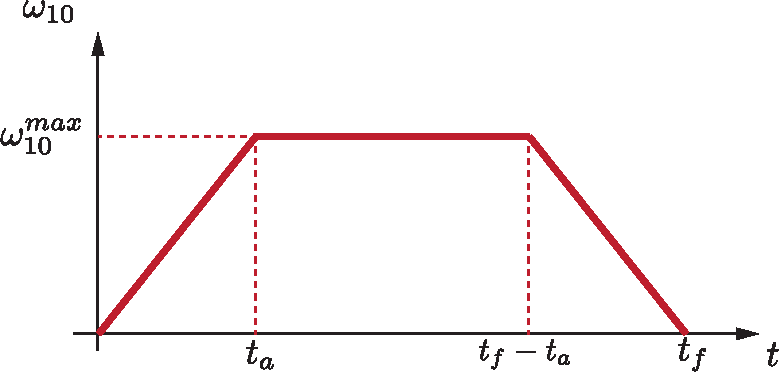
\includegraphics[width=.9\linewidth]{images/trapeze}
\end{center}
\end{minipage}
\begin{resultat}
Dans les 3 derniers points, il est souvent suffisant de remarquer en utilisant les courbes que : 
\begin{itemize}
\item $t_1=\dfrac{\dot{x}_m}{\ddot{x}_m}$;
\item en utilisant la courbe de vitesse et en remarquant que l'intégrale sous la courbe correspond à la distance parcourue, la distance parcourue lors de l'accélération est donnée par $\dfrac{1}{2}t_1\dot{x}_m$;
\item en utilisant la courbe de vitesse et en remarquant que l'intégrale sous la courbe correspond à la distance parcourue, la distance parcourue lors des 3 phases est donnée par $2\cdot \dfrac{1}{2}t_1\dot{x}_m+\left(t_2-t_1\right)\dot{x}_m$.
\end{itemize}
\end{resultat}


\begin{center}
\begin{tabular}{|p{2.2cm}|c|c|c|}
\hline
 & Phase 1 & Phase 2 & Phase 3 \\
\hline \hline
Équation de position & 
$x(t)=\dfrac{1}{2}\ddot{x}_mt^2 $ &
$x(t)= \dot{x}_m(t)\left( t-t_1\right)+x_m\left(t_1 \right)$ & 
$x(t)= -\dfrac{1}{2}\ddot{x}_m\left(t-t_2\right)^2 + \dot{x}_m(t)\left( t-t_2\right)+x_m\left(t_2\right)$ \\ \hline
Équation de vitesse &
$\dot{x}(t)=\ddot{x}_m t$ &  
$\dot{x}(t)=\dot{x}_m $ & 
$\dot{x}(t)=-\ddot{x}_m \left(t-t_2\right)+\dot{x}_m$  \\ \hline
Équation d'accélération &
$\ddot{x}(t)=\ddot{x}_m$ & 
$\ddot{x}(t)=0$ & 
$\ddot{x}(t)=-\ddot{x}_m$ \\
\hline
\end{tabular}
\end{center}

\begin{thebibliography}{2}
   \bibitem[1]{ref1} Émilien Durif, {\it Introduction à la dynamique des solides, Lycée La Martinière Monplaisir, Lyon.}
      \bibitem[2]{ref2} Florestan Mathurin, {\it Introduction à la dynamique du solide, Lycée Bellevue, Toulouse, \url{http://florestan.mathurin.free.fr/}.}
\end{thebibliography}

\end{document}



